\documentclass[
	12pt, % Default font size, values between 10pt-12pt are allowed
	%letterpaper, % Uncomment for US letter paper size
	%spanish, % Uncomment for Spanish
]{fphw}

% Template-specific packages
\usepackage[utf8]{inputenc} % Required for inputting international characters
\usepackage[T1]{fontenc} % Output font encoding for international characters
\usepackage{mathpazo} % Use the Palatino font
\usepackage{graphicx} % Required for including images
\usepackage{booktabs} % Required for better horizontal rules in tables
\usepackage{listings} % Required for insertion of code
\usepackage[shortlabels]{enumitem}





%----------------------------------------------------------------------------------------
%	ASSIGNMENT INFORMATION
%----------------------------------------------------------------------------------------

\title{Midterm} % Assignment title

\author{Zahin Mohammad \\ z5mohamm \\ 20669584} % Student name

\date{March 3rd, 2021} % Due date

\institute{University of Waterloo} % Institute or school name

\class{ECE 495} % Course or class name

\professor{Krzysztof Czarnecki} % Professor or teacher in charge of the assignment

% \begin{problem}
% TODO
% \end{problem}
% \subsection*{Answer}
% TODO
% \begin{center}
% 	\includegraphics[width=\columnwidth, page=1]{plot-a.pdf} % Example image
% \end{center}

%----------------------------------------------------------------------------------------
\begin{document}
\maketitle % Output the assignment title, created automatically using the information in the custom commands above
%----------------------------------------------------------------------------------------
%	ASSIGNMENT CONTENT
%----------------------------------------------------------------------------------------
\section*{Q1. ADS Fundamentals [1 mark]}
%------------------------------------------------
\begin{problem}
1a. A vehicle is equipped with a stop-and-go pilot, which can fully operate a vehicle on a
highway in traffic jams, but with a fallback-ready user. Which level(s) of driving
automation is this driving automation system operating at? [1 mark]
\end{problem}
\subsection*{Answer}
TODO
%----------------------------------------------------------------------------------------
\section*{Q2. Computer Vision Fundamentals [11 marks]}
%------------------------------------------------
\begin{problem}
2a. Compute 1-D cross-correlation by applying the following filter [0 2 1] to the
following signal [0 1 3 0] (assume enough zero padding to show all non-zero output). [2
		marks]
\end{problem}
\subsection*{Answer}
TODO
%------------------------------------------------
\begin{problem}
2b. Assume that the output of cross-correlating the 1-D filter [2 3 2] with some input
signal resulted in the following output signal [7 10 7]. What would be the output signal
have we used convolution instead of cross-correlation and why? [1 mark]
\end{problem}
\subsection*{Answer}
TODO
%------------------------------------------------
\begin{problem}
2c. What would be the result of applying this filter to an image (Hint: add the Gaussian
kernel to this filter from question 2e to recognize it)? [1 mark]Explain.
\begin{center}
	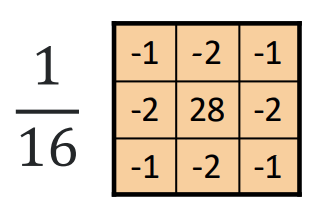
\includegraphics[width=0.5\columnwidth, page=1]{2c.png}
\end{center}
\end{problem}
\subsection*{Answer}
TODO
%------------------------------------------------
\begin{problem}
2d. What is the name of the following filter and what is it computing? [1 mark]
\begin{center}
	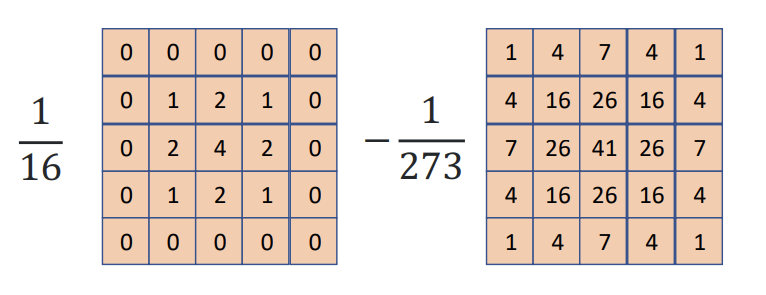
\includegraphics[width=0.5\columnwidth, page=1]{2d.png}
\end{center}
\end{problem}
\subsection*{Answer}
TODO
%------------------------------------------------
\begin{problem}
2e. Complete the Gaussian filter shown below by specifying the cells marked by “?”.
How did you determine the missing values? [2 marks]
\begin{center}
	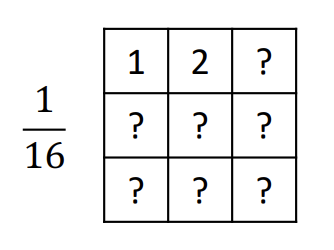
\includegraphics[width=0.5\columnwidth, page=1]{2e.png}
\end{center}
\end{problem}
\subsection*{Answer}
TODO
%------------------------------------------------
\begin{problem}
2f. Why is the Canny filter using double thresholding? [1 mark]
\end{problem}
\subsection*{Answer}
TODO
%------------------------------------------------
\begin{problem}
2g. Consider the following representation in Hough space (polar coordinates).
\begin{center}
	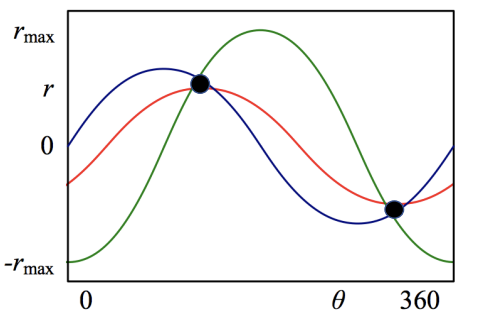
\includegraphics[width=0.5\columnwidth, page=1]{2g.png}
\end{center}
\begin{problem}
2g.1 What is each of the individual sinusoids corresponding to in the input image? [1
mark]
\end{problem}
\subsection*{Answer}
TODO
\begin{problem}
2g.2 What is each of the black dots (sinusoid intersections) corresponding to in the input
image (note that the horizontal axis sweeps 360 degrees)? [1 mark]
\end{problem}
\subsection*{Answer}
TODO
\end{problem}
%------------------------------------------------
\begin{problem}
2h. Which of the following value profiles represent black in HSV? (select all that apply)
[1 mark]
\begin{enumerate}
	\item 0,high,high
	\item any,low,low
	\item any,low,high
	\item 60,high,high
	\item any,high,low
	\item any,any,low
\end{enumerate}
\end{problem}
\subsection*{Answer}
TODO
%------------------------------------------------
%----------------------------------------------------------------------------------------
\section*{Q3. Machine Learning Fundamentals [21 marks]}

%------------------------------------------------
\begin{problem}
3a. Starting with the probabilistic model for linear regression (assume single input $x$ and
single out $y$), show that maximizing the likelihood for a dataset $(x,y)$ (with i.i.d.
datapoints) is equivalent to minimizing the sum of squared errors. Hint: go via negative
log likelihood [5 marks]
\end{problem}
\subsection*{Answer}
TODO
%------------------------------------------------
\begin{problem}
3b. What is the regression loss (as used in class) for a data point with label 0.4 and
predicted output 0.7? [1 mark]
\end{problem}
\subsection*{Answer}
TODO
%------------------------------------------------
\begin{problem}
3c. (Apply what you’ve learned in lecture and Assignment 2) Given the following set of
input vector $X$, ground truth vector $Y$, and weight matrices $W_1$, $W_2$, $B_1$, and $B_2$ of a 2
layer fully connected neural network, what is the inference probability of the correct
class? What is the cross-entropy loss value? Assume ReLU activation on the first hidden
layer and softmax activation on the output layer. Show each step of the computation.
Hint: Use numerically stable softmax and assume $e^{-1}) \approx 0.37$ and $e^{-7}\approx 0.00$ [5
		marks]
\begin{center}
	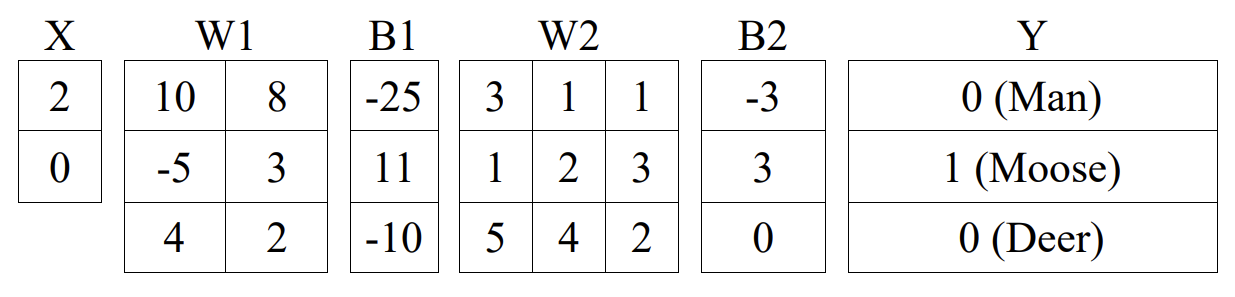
\includegraphics[width=0.75\columnwidth, page=1]{3c.png} % Example image
\end{center}
\end{problem}
\subsection*{Answer}
TODO
%------------------------------------------------
\begin{problem}
3d. Consider the computational graph below for the following function
\begin{equation}
	f(x_1, x_2) = ln(3x_1+e^{2x_2})
\end{equation}
Draw the computational graph and annotate it with the forward pass (above the arrows)
and backward pass (below the arrows) for $x_1=1$ and $x_2=0$ (propagate the gradient
back to each function input). Recall
\begin{equation}
	\frac{de^x}{dx} = e^x
\end{equation}
\begin{equation}
	\frac{dln(x)}{dx} = \frac{1}{x}
\end{equation}
Assume $ln(4) \approx 1.39$ [5 marks]
\end{problem}
\subsection*{Answer}
TODO
%------------------------------------------------
\begin{problem}
3e. What is the difference between Stochastic Gradient Descent and ordinary (Batch)
Gradient Descent? [1 mark]
\end{problem}
\subsection*{Answer}
TODO
%------------------------------------------------
\begin{problem}
3f. How is the condition of overfitting defined? [1 mark]
\end{problem}
\subsection*{Answer}
TODO
%------------------------------------------------
\begin{problem}
3g. Consider a convolutional layer with an input volume of depth 4 and output volume of
depth 128. How many convolutional filters does the layer contain? What is the depth of
each filter? [2 marks]
\end{problem}
\subsection*{Answer}
TODO
%----------------------------------------------------------------------------------------
\section*{Q4. Semantic Segmentation [2 marks]}
%------------------------------------------------
\begin{problem}
4a. (Apply what you’ve learned in lecture and Assignment 3) Semantic segmentation
architectures sometimes use skip connections from early feature maps of the feature
extractor to the corresponding-size upsampled maps in the decoder. What is the role of
these connections? [1 mark]
\end{problem}
\subsection*{Answer}
TODO
\begin{problem}
4b. (Assignment 3) You were recommended to use batch norm as part of your network.
Given a layer with the linear transformation and an activation function, where is the batch
norm operation normally applied? [1 mark]
\end{problem}
\subsection*{Answer}
TODO
%----------------------------------------------------------------------------------------
\section*{Q5. Object Detection [9 marks] }
%------------------------------------------------
\begin{problem}
5a. Assume that an object detector uses a 5-by-5 grid and 3 anchor boxes at each cell.
What is the maximum number of objects that the detector can detect? [1 mark]
\end{problem}
\subsection*{Answer}
TODO
\begin{problem}
5b. On a test set with a total of 4 of cars in the ground truth, a detector produced 3
bounding boxes with the following (score, IoU): (0.5,0.7), (0.7,0.8), (0.9, 0.2) (assume
that each returned bounding box overlaps with a different ground truth). Assuming a
score threshold of 0.6 and IoU threshold of 0.6, specify the number of TP, FP, and FN. [3
		marks]
\end{problem}
\subsection*{Answer}
TODO
\begin{problem}
5c. (Assignment 4) Consider the figure below, which shows the bounding boxes
predicted by a network (before non-maximum suppression). With an IoU threshold of 0.5
and detection threshold of 0.2, how many bounding boxes are left after non-maximal
suppression? Explain your reasoning. [3 marks]
\begin{center}
	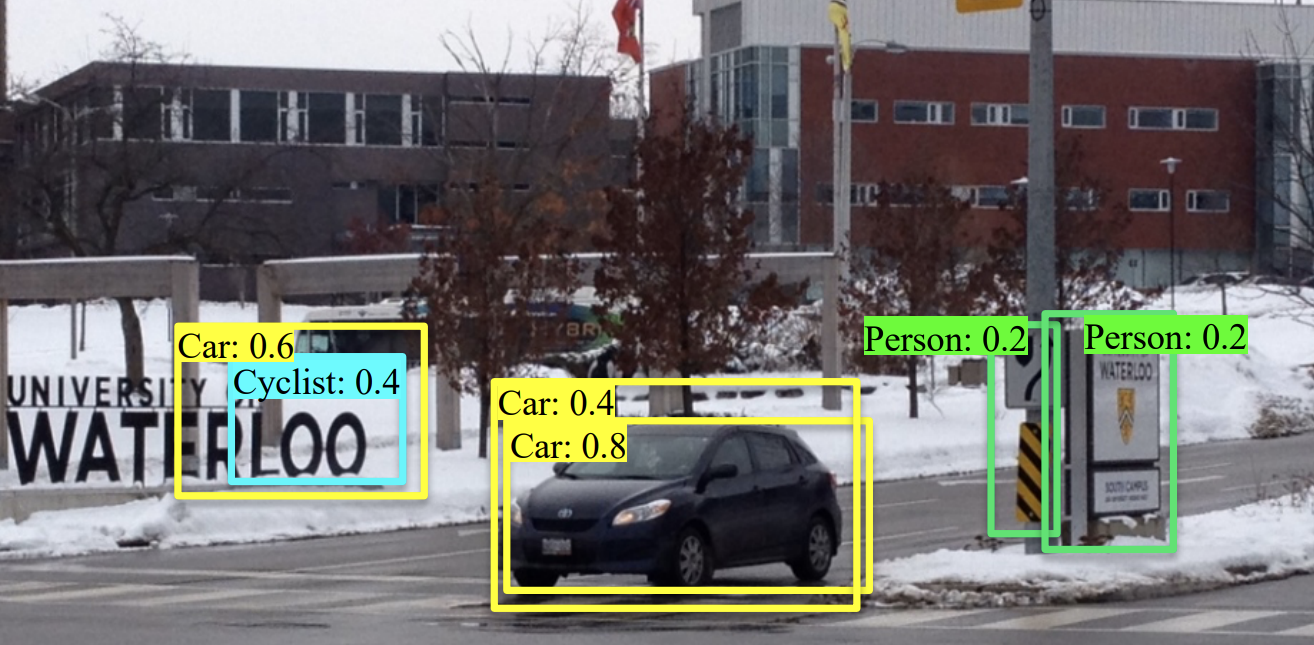
\includegraphics[width=0.75\columnwidth, page=1]{5c.png} % Example image
\end{center}
\end{problem}
\subsection*{Answer}
TODO
\begin{problem}
5d. How is it possible for two different bounding boxes to be generated for the same
object (before non-maximum suppression)? [1mark]
\end{problem}
\subsection*{Answer}
TODO
\begin{problem}
5e. Which of the statements is correct? [1mark]
\begin{enumerate}[a)] % a), b), c), ...
	\item An output neuron in an object detector is influenced only by input pixels within
	      the anchor box assigned to it.
	\item An output neuron in an object detector is influenced only by input pixels within
	      its positive anchor box.
	\item An output neuron in an object detector is influenced only by input pixels within
	      its empirical receptive field.
\end{enumerate}
\end{problem}
\subsection*{Answer}
TODO

\end{document}
